% the document class specification for the proposal writing process, add the 'submit' option
% for submitting (switches off various draft features); add the 'public' option to exclude
% any private parts. 
\documentclass[noworkareas,deliverables,gitinfo]{euproposal}
%\documentclass[submit,noworkareas,deliverables]{euproposal}
%\documentclass[submit,public,noworkareas,deliverables]{euproposal}
%% TODO these don't work with WA (https://trac.kwarc.info/sTeX/ticket/1697)
%\usepackage[T1]{fontenc}
%\usepackage[utf8]{inputenc}
\addbibresource{../lib/dummy}
%%% institutions
\WAinstitution[id=PS,
        countryshort=FR,
        acronym=UPSud]
        {Universit\'e Paris Sud}

\WAinstitution[id=LL,
        countryshort=FR,
        acronym=Logilab]
        {Logilab}

\WAinstitution[id=UV,
        countryshort=FR,
        acronym=UVSQ]
        {Universit\'e de Versailles Saint-Quentin}

\WAinstitution[id=UJF,
        countryshort=FR,
        acronym=UJF]
        {Universit\'e Joseph Fourier}

\WAinstitution[id=UB,
        countryshort=FR,
        acronym=CNRS]
        {CNRS}

\WAinstitution[id=UO,
        countryshort=UK,
        acronym=UO]
        {University of Oxford}

\WAinstitution[id=USH,
        countryshort=UK,
        acronym=USHEF]
        {University of Sheffield}

\WAinstitution[id=USO,
        countryshort=UK,
        acronym=USO]
        {University of Southampton}

\WAinstitution[id=SA,
        countryshort=UK,
        acronym=USTAN]
        {University of St Andrews}

\WAinstitution[id=UW,
        countryshort=UK,
        acronym=UW]
        {University of Warwick}

\WAinstitution[id=JU,
        countryshort=DE,
        acronym=JacU]
        {Jacobs University Bremen}

\WAinstitution[id=UK,
        countryshort=DE,
        acronym=UK]
        {University of Kaiserslautern}

\WAinstitution[id=US,
        countryshort=PL,
        acronym=US]
        {University of Silesia}

\WAinstitution[id=ZH,
        countryshort=CH,
        acronym=UZH]
        {Universit\"{a}t Z\"{u}rich}

\WAinstitution[id=SR,
        countryshort=NO,
        acronym=Simula]
        {Simula Research Laboratory}

% \WAinstitution[id=UWS,
%         countryshort=US,
%         acronym=UWS]
%         {University of Washington at Seattle}

% \WAperson[id=miko, 
%            personaltitle=Prof. Dr.,
%            birthdate=13. September 1964,
%            academictitle=Professor of Computer Science,
%            affiliation=jacu,
%            department=case,
%            privaddress=None of your business,
%            privtel=that neither,
%            email=m.kohlhase@jacobs-university.de,
%            workaddress={Campus Ring 1, 28757 Bremen},
%            worktel=+49 421 200 3140,
%            worktelfax=+49 421 200 3140/493140,
%            workfax=+49 421 200 493140]
%            {Michael Kohlhase}

\WAperson[id=thiery,
           personaltitle=Prof. ,
           birthdate=28 Mai 1973,
           academictitle=Professor of Computer Science,
           affiliation=PS,
           department=Laboratoire de Recherche en Informatique,
           privaddress=None of your business,
           privtel=that neither,
           email=Nicolas.Thiery@u-psud.fr,
           workaddress={Campus Ring 1, 28757 Bremen},
           %worktel=+33 6 77 90 32 79,
           worktelfax=+33 6 77 90 32 79,
           %workfax=N/A
           ]
           {Nicolas M. Thiéry}

%%% Local Variables: 
%%% mode: latex
%%% TeX-master: "proposal"
%%% End: 

% LocalWords:  WAperson miko personaltitle academictitle privaddress privtel Sud
% LocalWords:  workaddress worktel workfax gc worktelfax pcg pcsa WAinstitution
% LocalWords:  shortname partof streetaddress townzip countryshort efo 3kd89
% LocalWords:  jacobs-logo.png Seefahrtstrasse Kruislann Montparnasse Universit
% LocalWords:  baz Westerfield
% Some sections of the included files depend on this.


\begin{document}
\begin{center}\color{red}\huge
This mock proposal is just an example for \texttt{euproposal.cls} it reflects the ICT
template of May 2011
\end{center}
\begin{proposal}[site=jacu,jacuRM=36,
  site=efo,efoRM=36,
  site=bar,barRM=36,
  site=baz,bazRM=36,
  coordinator=miko,
  acronym={iPoWr},
  acrolong={\underline{I}ntelligent} {\underline{P}r\underline{o}sal} {\underline{Wr}iting},
  title=\pn: \protect\pnlong,
  callname = ICT Call 1,
  callid = FP7-???-200?-?,
  instrument= Small or Medium-Scale Focused Research Project (STREP), 
  challengeid = 4,
  challenge = ICT for EU Proposals,
  objectiveid={ICT-2012.4.4}, 
  objective = Technology-enhanced Documents,
  outcomeid = b1,
  outcome = {More time for Research, not Proposal writing},
  coordinator=miko,
  months=24,
  compactht]
\begin{abstract}
  Writing grant proposals is a collaborative effort that requires the integration of
  contributions from many individuals. The use of an ASCII-based format like {\LaTeX}
  allows to coordinate the process via a source code control system like
  {\textsc{Subversion}}, allowing the proposal writing team to concentrate on the contents
  rather than the mechanics of wrangling with text fragments and revisions.
\end{abstract}

\tableofcontents

\begin{todo}{from the proposal template}
  Recommended length for the whole part B: 50--60 pages (including tables, references,
  etc.)
\end{todo}
\chapter{Scientific and Technical Quality}\label{chap:quality}
\begin{todo}{from the proposal template}
  Maximum length for the whole of Section 1 –-- twenty pages, not including the tables in
  Section 1.3
\end{todo}

\section{Targeted breakthrough and long-term vision}\label{sec:objectives}
\begin{todo}{from the proposal template}
  Describe the breakthrough(s) that you are targeting to achieve. What is the long-term
  vision (scientific, technological, societal, other) that motivates this breakthrough?
  Explain how this breakthrough is an essential step towards the achievement of your
  long-term vision, in particular in terms of new forms and uses of information and
  information technologies. Describe the concrete objectives that you consider to
  constitute the proof-of-concept of such a breakthrough. The objectives should be those
  that you consider achievable within the project, in spite of the inherent risks. They
  should be stated in a verifiable form, including through the milestones that will be
  indicated under Section 1.3 below.
\end{todo}

%%% Local Variables: 
%%% mode: latex
%%% TeX-master: "propB"
%%% End: 

\section{Novelty and foundational character}\label{sec:progress}
\begin{todo}{from the proposal template}
  Describe the state-of-the-art in the area(s) concerned, and the advance that the
  proposed project would bring about. Clearly describe the novelty of your proposal. In
  what way do you challenge current thinking or assumptions? Novelty should come from new
  ideas, not from the incremental refinement of existing approaches. It can also come from
  new and unexpected combinations of insights from various disciplines. What is the
  scientific foundation that you aim to develop and what are the specific contributions to
  science and technology that your project will make (including in case of failure)?
\end{todo}

%%% Local Variables: 
%%% mode: latex
%%% TeX-master: "propB"
%%% End: 

\section{Scientific/Technical Methodology and Work Plan}\label{sec:methodology}
\begin{todo}{from the proposal template}
  A detailed work plan should be presented, broken down into work packages\footnote{A work
    package is a major sub-division of the proposed project with a verifiable end-point –
    normally a deliverable or an important milestone in the overall project.} (WPs) which
  should follow the logical phases of the implementation of the project, and include
  consortium management and assessment of progress and results. (Note that your overall
  approach to management will be described later, in Section 2).

Notes: The number of work packages used must be appropriate to the complexity of the work
and the overall value of the proposed project. The planning should be sufficiently
detailed to justify the proposed effort and allow progress monitoring by the Commission.

Any significant risks should be identified, and contingency plans described
\end{todo}
\newpage\begin{todo}{from the proposal template}
\begin{enumerate}
\item Describe the overall strategy of the work plan\ednote{Maximum length – one page}
\item Show the timing of the different WPs and their components (Gantt chart or similar).
\end{enumerate}
\end{todo}
\begin{figure}
  \caption{Work package dependencies}
  \label{fig:wp-deps}
\end{figure}

\ganttchart[draft,xscale=.45] 

%%% Local Variables: 
%%% mode: LaTeX
%%% TeX-master: "propB"
%%% End: 

% LocalWords:  workplan.tex ednote wp-deps ganttchart xscale


\newpage
\subsection{Work Package List}\label{sec:wplist}

\begin{todo}{from the proposal template}
Please indicate one activity per work package:
RTD = Research and technological development; DEM = Demonstration; MGT = Management of the consortium
\end{todo}

%\makeatletter\wp@total@RM{management}\makeatother
\wpfigstyle{\footnotesize}
\wpfig[pages,type,start,end]

\newpage%% Deliverables list.
%% Deliverables ordered by Workpackage
%% Workpackages are numbered automatically in sequence - the WP number has no effect

\workpackage{1}{Project Management}
\deliverable{mgt:mailinglists}
\deliverable{mgt:projectwebsite}
\deliverable{mgt:swrepository}
\deliverable{mgt:periodic-rep-1}
\deliverable{mgt:periodic-rep-2}
\deliverable{mgt:periodic-rep-3}
\deliverable{mgt:periodic-rep-4}
\deliverable{mgt:final-mgt-rep}
% Metrics: in PM and a bit in each work package

\workpackage{2}{Community Building and Engagement}
\deliverable{del:xx}

\workpackage{3}{Component Architecture}
\deliverable{del:xx}

%\workpackage{XXX}{Standardization} % => Component architecture + advertisement in the dissemination
%\deliverable{del:xx}

\workpackage{4}{User Interfaces}
\deliverable{del:xx}

\workpackage{5}{HPC and massively parallel components}
\deliverable{del:xx}

\workpackage{6}{Next generation Mathematical Databases}
\deliverable{del:xx}
%SL

\workpackage{7}{Development Models for an Academic Free Software Ecosystem}
\deliverable{del:xx}
%SL? Dima?

\workpackage{8}{Social Aspects}
\deliverable{del:xx}
%UM
%\workpackage{XXX}{Supporting the Mathematical Process} % => A chunk of Social Aspects
%\deliverable{del:xx}


\workpackage{9}{Dissemination, Exploitation and Communication}
\deliverable{del:pressrelease} % Press release.
\deliverable{del:website} % Project presentation (web site). 
\deliverable{del:workshop1}  % Report on first project workshop, year 1. 
\deliverable{del:dissemplan1} % Final plan for using and disseminating knowledge.
\deliverable{del:workshop2}  % Report on second project workshop, year 2
\deliverable{del:workshop3}  % Report on third project workshop, year 3
\deliverable{del:dissemplan2} % Final plan for using and disseminating knowledge.

\newpage\eucommentary{Milestones means control points in the project that help to chart progress. Milestones may
correspond to the completion of a key deliverable, allowing the next phase of the work to begin.
They may also be needed at intermediary points so that, if problems have arisen, corrective
measures can be taken. A milestone may be a critical decision point in the project where, for
example, the consortium must decide which of several technologies to adopt for further
development.}

The work in the \TheProject project is structured by four milestones,
which coincide with the four project meetings held at the end of each
year of the project (the other four meetings will be held in the middle
of each year). Given the nature of the project, with a
large number of essentially independent tasks, there is no need for
milestones attached to specific collections of tasks or
deliverables. Instead, given that the meetings are the main
face-to-face interaction points in the project, it's suitable to
schedule the milestones for these events, where they can be discussed
in detail, tracking the progress in each work package through status
reports on the tasks and deliverables.

We envisage that this setup will give the project the vital coherence
in spite of the broad interdisciplinary mix of various backgrounds of the
participants.

% \newcommand{\WPall}{\WPref{management}, \WPref{dissem}, \WPref{component-architecture}, \WPref{UI}, \WPref{hpc}, \WPref{dksbases}, \WPref{social-aspects}}

% \newcommand{\WPnoUI}{\WPref{management}, \WPref{dissem}, \WPref{component-architecture}, \WPref{hpc}, \WPref{dksbases}, \WPref{social-aspects}}

% \begin{center}
%   \begin{tabular}{|m{.05\textwidth}|m{.30\textwidth}|m{.15\textwidth}|m{.05\textwidth}|m{.22\textwidth}|}
%     \hline
%     Mile-stone nr. & Milestone name & Related work packages & Est. date & Means of verification \\\hline
%     M1 & Requirements study, design and prototype implementations. Start of
%          community building.
%        & \WPall 
%        & 12 
%        & 2nd Project meeting report. Completion of corresponding deliverables. \\\hline
%     M2 & First fully functional interface implementations.
%          Enhanced versions of \TheProject components.
%          Training early adopters.
%        & \WPall 
%        & 24 
%        & 4th Project meeting report. Completion of corresponding deliverables. \\\hline
%     M3 & Evaluating \TheProject software. Working with the community 
%          and building portfolio of experiments produced with \TheProject.
%        & \WPall 
%        & 36 
%        & 6th Project meeting report. Completion of corresponding deliverables. \\\hline
%     M4 & Project evaluation and final versions of all \TheProject components.
%        & \WPnoUI 
%        & 48 
%        & 8th Project meeting report. Completion of corresponding deliverables. \\\hline
%   \end{tabular}
% \end{center}

\begin{milestones}
  \milestone[id=startup,month=12,
  verif={Completed all corresponding deliverables and reported the progress in the 2nd Project meeting report.}]
  {Startup}
  {By Milestone 1 we will have carried out the requirements study, design and prototype implementations and started community building activities.}

  \milestone[id=proto1,month=24,
  verif={Completed all corresponding deliverables and reported the progress in the 4th Project meeting report.}]
  {Prototypes}
  {By Milestone 2 we will have constructed first fully functional interface implementations and released enhanced versions of \TheProject components, and train early adopters of \TheProject.}

  \milestone[id=community,month=36,
  verif={Completed all corresponding deliverables and reported the progress in the 6th Project meeting report.}]
  {Community/ Experiments}
  {By Milestone 3 we will have gathered and evaluated feedback on \TheProject software and established the portfolio of experiments produced with \TheProject through further engaging with the community.}

  \milestone[id=eval,month=48,
  verif={Completed all corresponding deliverables and reported the progress in the 8th Project meeting report.}]
  {Evaluation}
  {By Milestone 4 we will have released final versions of all \TheProject components and completed the project evaluation.}
\end{milestones}

%%% Local Variables:
%%% mode: latex
%%% TeX-master: "proposal"
%%% End:

%  LocalWords:  verif ldots


\subsection{Work Package Descriptions}\label{sec:workpackages}
\begin{workplan}
\begin{workpackage}[id=management,type=MGT,wphases=0-24!.2,
  title=Project Management,short=Management,
  jacuRM=2,barRM=2,efoRM=2,bazRM=2]
We can state the state of the art and similar things before the summary in the boxes
here. 
\wpheadertable
\begin{wpobjectives}
  \begin{itemize}
    \item To perform the administrative, scientific/technical, and financial
      management of the project
    \item To co-ordinate the contacts with the EU
    \item To control quality and timing of project results and to resolve conflicts
    \item To set up inter-project communication rules and mechanisms
  \end{itemize}
\end{wpobjectives}

\begin{wpdescription}
  Based on the Consortium Agreement, i.e. the contract with the European Commission, and
  based on the financial and administrative data agreed, the project manager will carry
  out the overall project management, including administrative management.  A project
  quality handbook will be defined, and a {\pn} help-desk for answering questions about
  the format (first project-internal, and after month 12 public) will be established. The
  project management will\ldots we can even reference deliverables:
  \delivref{management}{report2} and even the variant with a title:
  \delivtref{management}{report2}
\end{wpdescription}

\begin{wpdelivs}
  \begin{wpdeliv}[due=1,id=mailing,nature=O,dissem=PP,miles=kickoff]
    {Project-internal mailing lists}
  \end{wpdeliv}
  \begin{wpdeliv}[due=3,id=handbook,nature=R,dissem=PU,miles=consensus]
    {Project management handbook}
  \end{wpdeliv}
\begin{wpdeliv}[due={6,12,18,24,30,36,42,48},id=report2,nature=R,dissem=public,miles={consensus,final}]
  {Periodic activity report} 
  Partly compiled from activity reports of the work package
  coordinators; to be approved by the work package coordinators before delivery to the
  Commission.  Financial reporting is mainly done in months 18 and 36.\Ednote{how about
    these numbers?}
  \end{wpdeliv}
 \begin{wpdeliv}[due=6,id=helpdesk,dissem=PU,nature=O,miles=kickoff]
    {{\pn} Helpdesk}
  \end{wpdeliv}
  \begin{wpdeliv}[due=36,id=report6,nature=R,dissem=PU,miles=final]
    {Final plan for using and disseminating the knowledge}
  \end{wpdeliv}
  \begin{wpdeliv}[due=48,id=report7,nature=R,dissem=PU,miles=final]
    {Final management report}
  \end{wpdeliv}
\end{wpdelivs}
\end{workpackage}

%%% Local Variables: 
%%% mode: LaTeX
%%% TeX-master: "propB"
%%% End: 

% LocalWords:  wp-management.tex workpackage efoRM bazRM wpheadertable pn ldots
% LocalWords:  wpobjectives wpdescription delivref delivtref wpdelivs wpdeliv
% LocalWords:  dissem Ednote pdataRef deliv mansubsusintReport wphases
\newpage
\begin{workpackage}%
[id=dissem,type=RTD,lead=efo,
 wphases=10-24!1,
 title=Dissemination and Exploitation,short=Dissemination,
 efoRM=8,jacuRM=2,barRM=2,bazRM=2]
We can state the state of the art and similar things before the summary in the boxes
here. 
\wpheadertable

\begin{wpobjectives}
  Much of the activity of a project involves small groups of nodes in joint work. This
  work package is set up to ensure their best wide-scale integration, communication, and
  synergetic presentation of the results. Clearly identified means of dissemination of
  work-in-progress as well as final results will serve the effectiveness of work within
  the project and steadily improve the visibility and usage of the emerging semantic
  services.
\end{wpobjectives}

\begin{wpdescription}
  The work package members set up events for dissemination of the research and
  work-in-progress results for researchers (workshops and summer schools), and for
  industry (trade fairs). An in-depth evaluation will be undertaken of the response of
  test-users.

  Within two months of the start of the project, a project website will go live. This
  website will have two areas: a members' area and a public area.\ldots
\end{wpdescription}

\begin{wpdelivs}
  \begin{wpdeliv}[due=2,id=website,nature=O,dissem=PU,miles=kickoff]
     {Set-up of the Project web server}
   \end{wpdeliv}
   \begin{wpdeliv}[due=8,id=ws1proc,nature=R,dissem=PU,miles={kickoff}]
     {Proceedings of the first {\pn} Summer School.}
   \end{wpdeliv}
   \begin{wpdeliv}[due=9,id=dissem,nature=R,dissem=PP]
     {Dissemination Plan}
   \end{wpdeliv}
   \begin{wpdeliv}[due=9,id=exploitplan,nature=R,dissem=PP,miles=exploitation]
     {Scientific and Commercial Exploitation Plan}
   \end{wpdeliv}
   \begin{wpdeliv}[due=20,id=ws2proc,nature=R,dissem=PU,miles={exploitation}]
     {Proceedings of the second {\pn} Summer School.}
   \end{wpdeliv}
   \begin{wpdeliv}[due=32,id=ss1proc,nature=R,dissem=PU,miles={exploitation}]
     {Proceedings of the third {\pn} Summer School.}
   \end{wpdeliv}
   \begin{wpdeliv}[due=44,id=ws3proc,nature=R,dissem=PU,miles=exploitation]
     {Proceedings of the fourth {\pn} Summer School.}
   \end{wpdeliv}
 \end{wpdelivs}
\end{workpackage}

%%% Local Variables: 
%%% mode: LaTeX
%%% TeX-master: "propB"
%%% End: 

% LocalWords:  wp-dissem.tex workpackage dissem efo fromto bazRM wpheadertable
% LocalWords:  wpobjectives wpdescription ldots wpdelivs wpdeliv ws1proc pn
% LocalWords:  exploitplan ws2proc ss1proc ws3proc pdataRef deliv
% LocalWords:  mansubsusintReport
\newpage
\begin{workpackage}[id=class,type=RTD,lead=jacu,
                    wphases=3-9!1,
                    title=A {\LaTeX} class for EU Proposals,short=Class,
                    jacuRM=12,barRM=12]
We can state the state of the art and similar things before the summary in the boxes
here. 
\wpheadertable
\begin{wpobjectives}
\LaTeX is the best document markup language, it can even be used for literate
programming~\cite{DK:LP,Lamport:ladps94,Knuth:ttb84}

  To develop a {\LaTeX} class for marking up EU Proposals
\end{wpobjectives}

\begin{wpdescription}
  We will follow strict software design principles, first comes a requirements analys,
  then \ldots
\end{wpdescription}

\begin{wpdelivs}
  \begin{wpdeliv}[due=6,id=req,nature=R,dissem=PP,miles=kickoff]
     {Requirements analysis}
   \end{wpdeliv}
   \begin{wpdeliv}[due=12,id=spec,nature=R,dissem=PU,miles=consensus]
     {{\pn} Specification }
   \end{wpdeliv}
   \begin{wpdeliv}[due=18,id=demonstrator,nature=P,dissem=PU,miles={consensus,final}]
     {First demonstrator ({\tt{article.cls}} really)}
   \end{wpdeliv}
   \begin{wpdeliv}[due=24,id=proto,nature=P,dissem=PU,miles=final]
     {First prototype}
   \end{wpdeliv}
    \begin{wpdeliv}[due=36,id=release,nature=P,dissem=PU,miles=final]
      {Final {\LaTeX} class, ready for release}
    \end{wpdeliv}
  \end{wpdelivs}
Furthermore, this work package contributes to {\pdataRef{deliv}{managementreport2}{label}} and
{\pdataRef{deliv}{managementreport7}{label}}.
\end{workpackage}

%%% Local Variables: 
%%% mode: LaTeX
%%% TeX-master: "propB"
%%% End: 
\newpage
\begin{workpackage}[id=temple,type=DEM,lead=bar,
  wphases=6-12!1,
  title={\pn} Proposal Template,short=Template,barRM=6,bazRM=6]
We can state the state of the art and similar things before the summary in the boxes
here. 
\wpheadertable

\begin{wpobjectives}
  To develop a template file for {\pn} proposals
\end{wpobjectives}

\begin{wpdescription}
  We abstract an example from existing proposals
\end{wpdescription}

\begin{wpdelivs}
  \begin{wpdeliv}[due=6,id=req,nature=R,dissem=PP,miles=kickoff]
    {Requirements analysis}
  \end{wpdeliv}
  \begin{wpdeliv}[due=12,id=spec,nature=R,dissem=PU,miles=consensus]
    {{\pn} Specification }
  \end{wpdeliv}
  \begin{wpdeliv}[due=18,id=demonstrator,nature=D,dissem=PU,miles={consensus,final}]
    {First demonstrator ({\tt{article.cls}} really)}
  \end{wpdeliv}
  \begin{wpdeliv}[due=24,id=proto,nature=P,dissem=PU,miles=final]
    {First prototype}
  \end{wpdeliv}
  \begin{wpdeliv}[due=36,id=release,nature=P,dissem=PU,miles=final]
    {Final Template, ready for release}
  \end{wpdeliv}
\end{wpdelivs}
Furthermore, this work package contributes to {\pdataRef{deliv}{managementreport2}{label}} and
{\pdataRef{deliv}{managementreport7}{label}}.
\end{workpackage}

%%% Local Variables: 
%%% mode: LaTeX
%%% TeX-master: "propB"
%%% End: 

% LocalWords:  wp-temple.tex workpackage fromto pn bazRM wpheadertable wpdelivs
% LocalWords:  wpobjectives wpdescription wpdeliv req dissem tt article.cls
% LocalWords:  pdataRef deliv systemsintReport
\newpage
\end{workplan}
\newpage\subsection{Significant Risks and Associated Contingency Plans}\label{sec:risks}
\begin{todo}{from the proposal template}
  Describe any significant risks, and associated contingency plans
\end{todo}
\begin{oldpart}{need to integrate this somewhere. CL: I will check other proposals to see how they did it; the Guide does not really prescribe anything.}
\paragraph{Global Risk Management}
The crucial problem of \pn (and similar endeavors that offer a new basis for communication
and interaction) is that of community uptake: Unless we can convince scientists and
knowledge workers industry to use the new tools and interactions, we will
never be able to assemble the large repositories of flexiformal mathematical knowledge we
envision. We will consider uptake to be the main ongoing evaluation criterion for the network.
\end{oldpart}

%%% Local Variables: 
%%% mode: latex
%%% TeX-master: "propB"
%%% End: 



%%% Local Variables: 
%%% mode: latex
%%% TeX-master: "propB"
%%% End: 

% LocalWords:  workplan newpage wplist makeatletter makeatother wpfig
% LocalWords:  workpackages wp-dissem wp-class wp-temple

%%% Local Variables: 
%%% mode: LaTeX
%%% TeX-master: "propB"
%%% End: 

\newpage
\chapter{Implementation}\label{chap:implementation}

\section{Management Structure and Procedures}\label{chap:management}
\begin{todo}{from the proposal template}
  Describe the organizational structure and decision-making mechanisms
  of the project. Show how they are matched to the nature, complexity
  and scale of the project.  Maximum length of this section: five pages.
\end{todo}

The Project Management of {\pn} is based on its Consortium Agreement, which will be
signed before the Contract is signed by the Commission. The Consortium Agreement will
enter into force as from the date the contract with the European Commission is signed.
\subsection{Organizational structure}\label{sec:management-structure}
\subsection{Risk Assessment and Management}
\subsection{Information Flow and Outreach}\label{sec:spread-excellence}
\subsection{Quality Procedures}\label{sec:quality-management}
\subsection{Internal Evaluation Procedures}
\newpage
\section{Individual Participants}\label{sec:partners}
\begin{todo}{from the proposal template}
For each participant in the proposed project, provide a brief description of the legal entity, the main
tasks they have been attributed, and the previous experience relevant to those tasks. Provide also a
short profile of the individuals who will be undertaking the work.\\
Maximum length for Section 2.2: one page per participant. However, where two or more departments within
an organisation have quite distinct roles within the proposal, one page per department is acceptable.\\
The maximum length applying to a legal entity composed of several members, each of which is a separate
legal entity (for example an EEIG1), is one page per member, provided that the members have quite distinct
roles within the proposal.
\end{todo}
\newpage
\begin{sitedescription}{jacu}

\paragraph{Organization} Jacobs University Bremen is a private research university patterned
after the Anglo-Saxon university system.  The university opened in
2001 and has an international student body ($1,245$ students from 102
nations as of 2011, admitted in a highly selective process).

The KWARC (KnoWledge Adaptation and Reasoning for
Content\footnote{\url{http://kwarc.info}}) Group headed by
{\emph{Prof.\ Dr.\ Michael Kohlhase}} specializes in building
knowledge management systems for e-science applications, in particular
for the natural and mathematical sciences.  Formal logic, natural
language semantics, and semantic web technology provide the
foundations for the research of the group.
  
  Since doing research and developing systems is much more fun than writing proposals,
  they try go do that as efficiently as possible, hence this meta-proposal. 

\paragraph{Main tasks}

\begin{itemize}
\item creating {\LaTeX} class files
\end{itemize}

\paragraph{Relevant previous experience}

The KWARC group is the main center and lead implementor of the OMDoc
(Open Mathematical Document) format for representing mathematical
knowledge.  The group has developed added-value services powered by such semantically rich representations, different paths to obtaining them, as well as platforms that integrate both aspects.  Services include the adaptive context-sensitive presentation framework JOMDoc and the semantic search engine MathWebSearch.  For obtaining rich mathematical content, the group has been pursuing the two alternatives of assisting manual editing (with the sTeXIDE editing environment) and automatic annotation using natural language processing techniques.  The latter is work in progress but builds on the arXMLiv system, which is currently capable of converting 70\% out of the 600,000 scientific publications in the arXiv from {\LaTeX} to XHTML+MathML without errors.  Finally, the KWARC group has been developing the Planetary integrated environment.

\paragraph{Specific expertise}

\begin{itemize}
\item writing intelligent proposals
\end{itemize}

\paragraph{Staff members involved}

\textbf{Prof.\ Dr.\ Michael Kohlhase} is head of the KWARC research
group.  He is the head developer of the OMDoc mathematical markup
language.  He was a member of the Math Working Group at W3C, which finished its work with the publication of the MathML 3 recommendation.  He is president of the OpenMath society and trustee of the MKM
interest group.

\keypubs{KohDavGin:psewads11,Kohlhase:pdpl10,Kohlhase:omdoc1.2,CarlisleEd:MathML10,StaKoh:tlcspx10}
\end{sitedescription}

%%% Local Variables: 
%%% mode: LaTeX
%%% TeX-master: "propB"
%%% End: 

% LocalWords:  site-jacu.tex sitedescription emph textbf keypubs KohDavGin
% LocalWords:  psewads11 pdpl10 StaKoh tlcspx10
\newpage
\begin{sitedescription}{efo}
\paragraph{Organization}
 The EFO is the world leader in futurology, \ldots
\paragraph{Main tasks}
\paragraph{Relevant previous experience}
\paragraph{Specific expertise}
\paragraph{Staff members undertaking the work}
\keypubs{providemore}
\end{sitedescription}

%%% Local Variables: 
%%% mode: LaTeX
%%% TeX-master: "propB"
%%% End: 
\newpage
\begin{sitedescription}{bar}

\paragraph{Organization}
  Universit\'e de BAR specializes on drinking lots of red wine. It is a partner in the
  consortium, because it has a very nice chateau on the Cote d'Azure, where it can host
  gorgeous project meetings.

\paragraph{Main tasks}
\paragraph{Relevant previous experience}
\paragraph{Specific expertise}
\paragraph{Staff members undertaking the work}
\keypubs{providemore}

\end{sitedescription}

%%% Local Variables: 
%%% mode: LaTeX
%%% TeX-master: "propB"
%%% End: 
\newpage
\begin{sitedescription}{baz}
\paragraph{Organization}
\paragraph{Main tasks}
\paragraph{Relevant previous experience}
\paragraph{Specific expertise}
\paragraph{Staff members undertaking the work}
\keypubs{providemore}
\end{sitedescription}

%%% Local Variables: 
%%% mode: LaTeX
%%% TeX-master: "propB"
%%% End: 
\newpage

\section{The {\protect\pn} consortium as a whole}
\begin{todo}{from the proposal template}
  Describe how the participants collectively constitute a consortium capable of achieving
  the project objectives, and how they are suited and are committed to the tasks assigned
  to them. Show the complementarity between participants. Explain how the composition of
  the consortium is well-balanced in relation to the objectives of the project.  

  If appropriate describe the industrial/commercial involvement to ensure exploitation of
  the results. Show how the opportunity of involving SMEs has been addressed
\end{todo}

The project partners of the \pn project have a long history of successful collaboration;
Figure~\ref{tab:collaboration} gives an overview over joint projects (including proposals) and
joint publications (only international, peer reviewed ones).

\jointorga{jacu,efo,baz}
\jointpub{efo,baz,jacu}
\jointproj{efo,bar}
\coherencetable

\subsection{Subcontracting}\label{sec:subcontracting}
\begin{todo}{from the proposal template}
  If any part of the work is to be sub-contracted by the participant responsible for it,
  describe the work involved and explain why a sub-contract approach has been chosen for
  it.
\end{todo}
\subsection{Other Countries}\label{sec:other-countries}
\begin{todo}{from the proposal template}
  If a one or more of the participants requesting EU funding is based outside of the EU
  Member states, Associated countries and the list of International Cooperation Partner
  Countries\footnote{See CORDIS web-site, and annex 1 of the work programme.}, explain in
  terms of the project’s objectives why such funding would be essential.
\end{todo}

\subsection{Additional Partners}\label{sec:assoc-partner}
\begin{todo}{from the proposal template}
  If there are as-yet-unidentified participants in the project, the expected competences,
  the role of the potential participants and their integration into the running project
  should be described
\end{todo}
\section{Resources to be Committed}\label{sec:resources}
\begin{todo}{from the proposal template}
Maximum length: two pages

Describe how the totality of the necessary resources will be mobilized, including any resources that
will complement the EC contribution. Show how the resources will be integrated in a coherent way,
and show how the overall financial plan for the project is adequate.

In addition to the costs indicated on form A3 of the proposal, and the effort shown in Section 1.3
above, please identify any other major costs (e.g. equipment). Ensure that the figures stated in Part B
are consistent with these.
\end{todo}

\subsection{Travel Costs and Consumables}\label{sec:travel-costs}
\subsection{Subcontracting Costs}
\subsection{Other Costs}

%%% Local Variables: 
%%% mode: LaTeX
%%% TeX-master: "propB"
%%% End: 

% LocalWords:  pn newpage site-jacu site-efo site-baz jointpub efo baz
% LocalWords:  jointproj coherencetable assoc-partner
\newpage
% ---------------------------------------------------------------------------
%  Section 2: Impact
% ---------------------------------------------------------------------------

\section{Impact}
\label{sec:impact}

\TOWRITE{Simula}{Hans Petter and Valeriya will make a second iteration on the impact section for Friday}

\subsection{Expected Impacts}

\eucommentary{Please be specific, and provide only information that applies
to the proposal and its objectives. Wherever possible, use quantified
indicators and targets.\\
Describe how your project will contribute to:\\
-- the expected impacts set out in the work programme, under the relevant topic
(including key performance indicators/metrics for monitoring results and impacts);\\
-- improving innovation capacity and the integration of new knowledge
(strengthening the competitiveness and growth of companies by developing
innovations meeting the needs of European and global markets; and, where
relevant, by delivering such innovations to the markets;\\
-- any other environmental and socially important impacts (if not already
covered above).\\
Describe any barriers/obstacles, and any framework conditions (such as
regulation and standards), that may determine whether and to what extent
the expected impacts will be achieved. (This should not include any risk
factors concerning implementation, as covered in section 3.2.)}

\subsubsection{Impacts as listed in the work programme}

The following table shows how \TheProject  addresses the specific impacts
listed in the work programme.

%\TOWRITE{NT}{Double check the table below: margins + where the checks
%  are in the measures to maximize impact}
\def\tmc#1{\hline\multicolumn{2}{|m{.94\textwidth}|}{\textbf{#1}}\\\hline}
\tablehead{}
\begin{supertabular}{|m{.47\textwidth}m{.47\textwidth}|}\hline
  \tmc{More effective collaborations between researchers}

  \TheProject will strengthen collaborations between European scientific community in
  different branches of mathematics, through a development of the common e-infrastracture
  by bringing together software and databases previously separated, and build links with
  scientific communities in other disciplines (biology, physics, astronomy) that will use
  this e-infrastructure. The scientific community will considerably increase, by
  integrating new actors both from academic and non academic sector. & Key performance
  indicators :
  \begin{compactenum}
  \item By the end of the project, the scientific community in mathematics using the tool
    will increase by X \%
  \item The scientific community in other disciplines (biology, physics) using the tool
    will increase by X\%
  \item Number of enterprises using the tool will increase by X\%
  \end{compactenum} \\\hline

  \tmc{Higher efficiency and creativity in research, higher productivity of researchers
    thanks to reliable and easy access to discovery, access and re-use of data}

  The development of a new integrated tool, replacing 3
    previously separated tools, a possibility of real time data sharing, data re-use and
    simultaneous working will allow an important gain in time and in efficiency, and, by
    consequence, higher productivity of researchers. Moreover, the exchange of best
    practice (such as regular audit of codes) will have an important impact on the quality
    of the research. Finally, the unique tool will allow considerably reducing the costs
    of further research.

 &

  Key performance indicators :
  \begin{compactenum}
\item The e-infrastructure developed by the end of the project will help reducing time of
  research by X\%\item The productivity of researchers will increase by X\%\item Thank to
  best practice exchange, the quality of research will considerably increase and number of
  errors will be reduced\item Better traceability of research \item Costs for research
  considerably reduced
\end{compactenum}
\\\hline
\tmc{Accelerated innovation in research via
an integrated access to digital research resources, tools and services
across disciplines and user communities}

An integrated access to digital research
resources and tools that \TheProject will provide will clearly help
accelerating innovation in research across disciplines and communities.

The integrated tool will meet the needs and help overcoming the
obstacles that are common to several disciplines impacted by the
project, and both to academic and non-academic research. Industrial
actors, actively involved into the project will directly benefit from
the project results. &

Key performance indicators :

\begin{compactenum}
\item Emergence of new, improved research methods in several disciplines
using the tool\item Resolution of series of problems proper to
industrial actors in several disciplines
\end{compactenum}
\\\hline

\tmc{Researchers able to process structured and qualitative data in virtual and/or ubiquitous workspaces}

\TheProject will enable researchers to process
different kind of  data thanks to an integrated tool interconnected
with databases. Efficient data storage will allow further exploitation
and  re-use of mathematics data for further calculations and thus make
data processing more efficient.

Le travail sur la sémantique de données est fait plus en amont.
 &
Key performance indicators :

Note E.S. – Nicolas, ici, j'ai du mal, car pas sure si on répond
vraiment à ce critère.\\\hline

\tmc{Increased take-up of collaborative research and data sharing by new disciplines,
  research communities and institutions}

The project will clearly enhance a take-up
of collaborative research and data sharing by and between new
disciplines and research communities. The communities already using the
parts of the tool, will be enlarged, involving more and more industrial
actors and young scientists.

By developing the tool, it will reinforce collaborations between
different branches of mathematics (both pure and applied). Once
developed, the tool will be opened for research in various disciplines,
such as biology, physics, astronomy etc. &
Key performance indicators :

\begin{compactenum}
\item Increased collaborations and data sharing between different communities in
  mathematics
\item Increased collaborations and data sharing between research communities in other
  disciplines
\item Increased number of users, enlarged research communities
\end{compactenum}
\\\hline
\end{supertabular}

\subsubsection{Improving innovation capacity and the integration of new knowledge}


 Innovations developed by \TheProject project will meet the needs of the
following ecosystem participants:

\begin{enumerate}
\item Device / module vendors: hardware manufacturers, equipment
manufacturers of smartphones, tablets, laptops;
\item Network providers: service providers, network infrastructure
vendors (Avaya, Juniper, Extreme, Cisco…)
\item Platform providers
\item Cloud service providers: Software-as-a-Service,
Platform-as-Service, Infrastructure-as-a-Service
\item Systeme integrators: end-to-end integration services and
value-added services (Accenture, HP, IBM…)
\item End users: research communities; IT, healthcare, education and
aeronautics stakeholders
\end{enumerate}
Industrial stakeholders will be directly involved into the project and
the VRE development, so that the tool will be exactly tailored to their
specific needs – that are the same that the scientific community ones.
Moreover, this will allow an early time-to-market and will facilitate
the technology uptake.

In the table below we have specified different market needs, and the
ways the project will address each of them :

Table XX

\begin{flushleft}
\tablehead{}
\begin{supertabular}{|m{.47\textwidth}|m{.47\textwidth}|}
\hline
\centering Needs of markets &
\centering\arraybslash How the project will address these needs\\\hline
Performance gain &
The tool will enable its users to combine functionality from XXX other
mathematical software programs and programming languages

{}-mainstream programming language Python?

{}-which compilers?\\\hline
Infrastructure capacity: newly built infrastructures with fast broadband
connections are well positioned for adoption &
\TheProject will allow different groups of users to work simultaneously, and
thus provide a considerably gain in efficiency.\\\hline
Lower cost of scaling  &
An open source architecture brings affordability: people and
organizations donate towards common goals, and small organizations can
gain access to equipment and research talent typically only afforded by
the largest firms. Resources integration will reduce considerably the
time and the costs of operations.\\\hline
Going beyond limitations of interconnect technology &
An open source architecture brings creativity (=the best minds to solve
a problem)\\\hline
Enabling new applications and features &
Through a series of links that will be created between previously
separated tools, and data interoperability, the VRE will enable new
applications and features\\\hline
Early time-to-market (TTM): companies are looking for solutions that
would improve the speed at which they can procure services to bypass
traditional information technology departments &
The speed of development will improve tremendously thanks to open
source. The implication of industrial stakeholders into the development
will allow to deliver a tool the suits the best to their needs, and
thus speed-up the time to market and technology uptake.\\\hline
Easy-to-use service: first-time experiences is crucial to gain
acceptance &
{}-Design? Ergonomie? Nice multiuser web-based graphical user interface

{}-integration with learning tools? (example : interactive whiteboard)

\TOWRITE{NT}{E.S: Nicolas, il faut réflechir à la façon de rendre l'outil
plus attractif pour la jeune génération (=future génération des
chercheurs), car c'est la génération Y qui va définir des standards
pour la suite  {}- donc  plus d'impact et à plus long terme. Réfléchis
à la possibilité de rendre l'outil accessible sur mobiles, tablettes
etc., mais aussi à la façon ``~intéressante~'' de l'enseigner.}\\\hline
\end{supertabular}
\end{flushleft}

\subsubsection{Other impacts (environmental and socially important impacts)}

\TODO{Neil: Can we not be more ambitious than simply replacing the other alternative? By working in an open way we should be able to achieve much more rapid deployment of ideas (like in the RADIANT project I mentioned above).} 

Here, our mission statement will be the same as for \Sage: to provide
a viable free open source alternative to \Magma, \Maple, \Mathematica
and \Matlab.

To make \TheProject a new reference, it is important to focus on the young
generation, which will be the future users.

Generation Y phenomenon:

\begin{compactenum}
\item generation Y accounts for 30\% of the total projected population
in 2025
\item key influencers to change in workplace habits
\item easy adaptability to technology -{\textgreater} collaborative work
would make them more productive
\item compulsion to check smartphones for emails, texts or social media
updates -{\textgreater} adoption of social networks.
\end{compactenum}
2.1.4. Potential barriers and framework conditions (such as regulation
and standards), that may determine whether and to what extent the
expected impacts will be achieved. (This should not include any risk
factors concerning implementation, as covered in section 3.2.)

The project does not arise any specific regulation issues; in the
unlikely event that new norms would appear during the project,
appropriate measures will be taken by the advisory board following
advice of relevant experts and standards agencies on national and EU
level.

\subsection{Measures to Maximise Impact}

\subsubsection{Dissemination and Exploitation of Results}
\label{subsubsect:dissemination}

\eucommentary{-- Provide a draft 'plan for the dissemination and exploitation
of the project's results'. The plan, which should be proportionate to the
scale of the project, should contain measures to be implemented both during
and after the project.\\
Dissemination and exploitation measures should address the full range
of potential users and uses including research, commercial, investment,
social, environmental, policy making, setting standards, skills and
educational training.\\
The approach to innovation should be as comprehensive as possible,
and must be tailored to the specific technical, market and organisational
issues to be addressed\\
-- Explain how the proposed measures will help to achieve the expected impact of the
project . Provide a draft business plan for financial sustainability as stated in the Part
E of the Specific features for Research Infrastructures of the Horizon 2020 European
Research Infrastructures (including e-Infrastructures) Work Programme 2014-2015.\\
-- Where relevant, include information on how the participants will
manage the research data generated and/or collected during the
project, in particular addressing the following issues:
What types of data will the project generate/collect? What
standards will be used? How will this data be exploited and/or
shared/made accessible for verification and re-use (If data cannot
be made available, explain why)? How will this data be curated and preserved?\\
-- Include information about any open source software used or developed by the
project.\\
You will need an appropriate consortium agreement to manage (amongst other things)
the ownership and access to key knowledge (IPR, data etc.). Where relevant,
these will allow you, collectively and individually, to pursue market opportunities
arising from the project's results.\\
The appropriate structure of the consortium to support exploitation is addressed
in section 3.3. \\
-- Outline the strategy for knowledge management and protection. Include measures to
provide open access (free on-line access, such as the ``green'' or ``gold'' model) to
peer-reviewed scientific publications which might result from the project.\\
Open access publishing (also called 'gold' open access) means that an article is
immediately provided in open access mode by the scientific publisher. The associated costs
are usually shifted away from readers, and instead (for example) to the university or
research institute to which the researcher is affiliated, or to the funding agency supporting
the research.\\
Self-archiving (also called ``green'' open access) means that the published article or the
final peer-reviewed manuscript is archived by the researcher - or a representative - in an
online repository before, after or alongside its publication. Access to this article is often -
but not necessarily - delayed (``embargo period''), as some scientific publishers may wish to
recoup their investment by selling subscriptions and charging pay-per-download/view fees
during an exclusivity period.}

Three types of impact are possible with our dissemination and
communication activities: (1) people or organizations are informed
about \TheProject; (2) people or organizations act and use our conclusions
or results; (3) people or organizations contribute and help to develop
or improve the research infrastructure. The second form of impact
supposes that parties understand the messages. The third form supposes
learning, which is a very high level of impact. In the following table,
we have listed how the proposed measures will help to achieve the
expected impact among our stakeholders and target audiences.

Table X.  Draft 'plan for the dissemination and exploitation of the
project's results'.

\begin{flushleft}
\tablehead{}
\begin{supertabular}{|m{2cm}|m{8cm}|l|l|l|}
\hline
Target users &
Measures during the project &
\multicolumn{3}{m{3.9129999cm}|}{Expected impact}\\\hline
 &
 &
(1) &
(2) &
(3)\\\hline
Scientific community in mathematics

(experienced researchers and PhD students) &
\begin{compactenum}
\item Recruitment for the project of specialists from industrial sector
and PhD students that are already a part of the community ;\item 10
technical workshops organized in the frame of \TheProject,  \item 10
scientific trainings/year,  \item Participation to
international conferences like FPSAC, ISSAC, ... (4), international congress of mathematical
software (1)\item Workshops ``Sage and women'' (1?)\item 10
publications in (social aspects) \item Software demonstration during
the conferences{\textgreater}publication\item 100 PhD students trained
and accessing the infrastructure\item Workshops for PhD students in
Africa
\end{compactenum}
 &
X

X

X

X &
X

X

X

X

X

X

X &
X

X

X

X

X

X\\\hline
Scientific community in other disciplines &
\begin{compactenum}
\item Direct implication of the representatives of those disciplines
into the project;\item Annual participation in Pycon international
conference\item X scientific trainings to other communities; \item News
in Nature and other editions in other disciplines (specify!)\item Up to
X PhD students trained on the tool in biology, physics etc.\item
Workshop ``~sage \& women~'' in USA{\textgreater} pour
IPython
\end{compactenum}
 &
X
 &
X
X
X
X
X
X
 &
X
X
X\\\hline
Policy makers &
Are not directly concerned by the tool, but can be informed via
international conferences and publications &
X &
 &
\\\hline
Industry &
\begin{compactenum}
\item Industrial stakeholders have common needs with academic
researchers. They bring to the project their specific competences and
human resources. They are actively involved into the workshops and
trainings (50\% of audience). The project aims the enlargement of the
community thanks notably to new industrial actors (including in other
disciplines and sectors). They will appropriate the tool by their
direct involvement into the project, by participation to the workshops,
trainings and conferences or by their usual information channels.\item
Annual participation in Pycon international conference\item
Certification by technology clusters
\end{compactenum}
 &
X &
X
X
X
 &
X\\\hline
Standartisation

agencies  &
\begin{compactenum}
\item At the end of the project,~after internal standartisation, the new
norms will be accorded with specialized agencies at national and EU
levels
\end{compactenum}
 &
 &
X &
\\\hline
Students &
\begin{compactenum}
\item 5 MooCs destined to master students.\item The tool will be used
for the elaboration of pedagogical documents, referenced on the
specific website\item The projects results will be integrated into
Master courses, and into teacher training courses
\end{compactenum}
 &
X
X
X
 &
X
X &
\\\hline
Civil society &
\begin{compactenum}
\item Results will be presented on the annual event “Worldwide meetings
of the free software”. This event generally touches upon all free
phenomena in the society, and involved various stakeholders, including
civil society actors.
\end{compactenum}
 &
X &
X &
\\\hline
Public at large &
\begin{compactenum}
\item Series of actions in high schools led by PhD students to raise
awareness of pupils, and especially girls, on mathematics research and
scientific careers\item Communication large public via annual events
like ``~Science holiday~'' etc.\item Vulgarization papers and
communication events addressed to people interested by ICT. \item Social
networks and platforms
\end{compactenum}
 &
X
X
X
X &
 &
\\\hline
\end{supertabular}
\end{flushleft}
Measures after the project:

\begin{compactenum}
\item Continue dissemination to scientific community and industrial
stakeholders through participation to international conferences (
FPSac, Isaac, Pycon, Sage and Women etc.) and publications
\item Software demonstration during the conferences
\item Training of  PhD students in mathematics, informatics and other
disciplines, both in Europe and all over the world
\item Large public communication  through regular vulgarization events
\end{compactenum}
Draft business plan for financial sustainability (as stated in the Part
E of the Specific features for Research Infrastructures of the Horizon
2020 European Research Infrastructures (including e-Infrastructures)
Work Programme 2014-2015).

\paragraph{Long term sustainability}

By design (Objective~\ref{objective:framework}), the VRE's promoted by
\TheProject will consist of a thin layer on top of an ecosystem of
components. Hence, the long term sustainability of those VRE is
guaranteed by the sustainability of the ecosystem of components, that
is by Objective~\ref{objective:sustainable}.

The needs in financial support after the end of the project are
therefore not very
important. We expect that a part of developers positions will be made
durable by the partners institutions, thanks to an increase of
awareness among them on the necessity of this infrastructure for their
own needs.

With the increase of the number of users, more and more research
laboratories, teaching institutions, and enterprises will get a need
for using this VRE – thus, additional funding will be possible through
access provision to other scientific communities, on projects base, or
via service delivery.
% This is already the business model chosen by \SMC.

\TODO{None of the two models below really match our situation;
  investigate for some good picture and language, e.g. in ``Economie
  du Logiciel Libre'' of François Élie}

Here we propose two possible models of this use:

\begin{figure}[ht]\centering
 \fbox{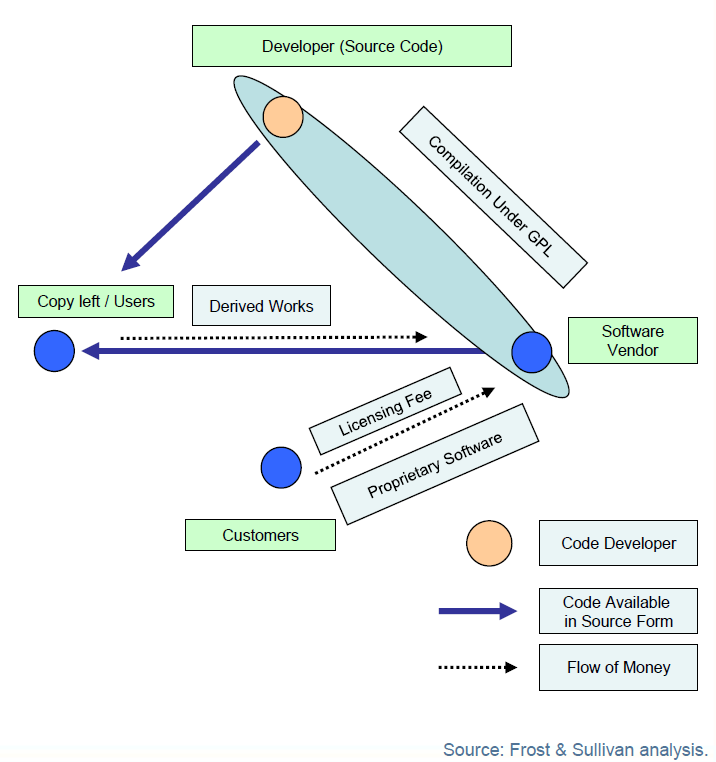
\includegraphics[width=.94\textwidth]{Impact-img1.png}}
 \caption{The GPL Model}\label{fig:gpl-model}
\end{figure}

\begin{figure}[ht]\centering
 \fbox{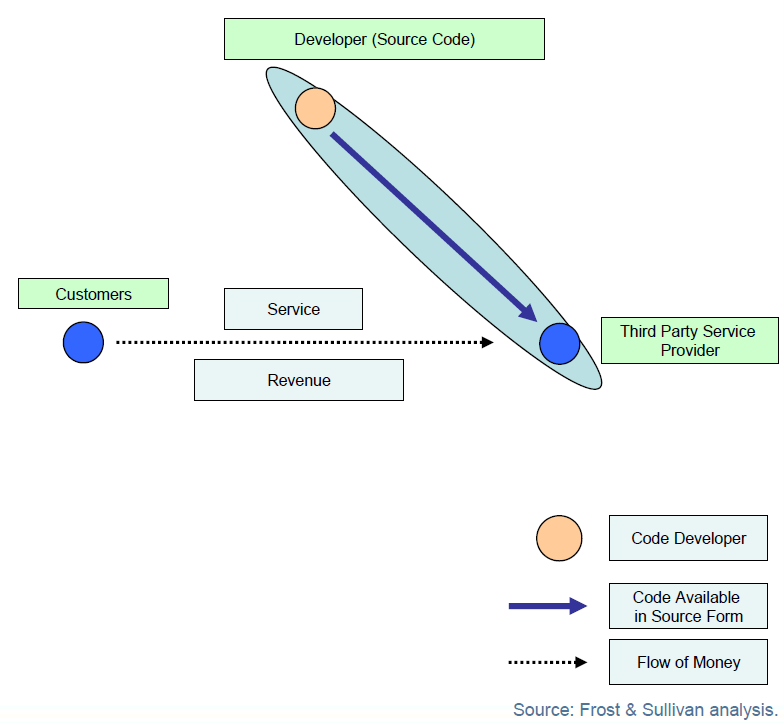
\includegraphics[width=.94\textwidth]{Impact-img2.png}}
 \caption{The Third-Party Services Model}\label{fig:tps-model}
\end{figure}

\begin{enumerate}
\item The \textbf{GPL model} (see Figure~\ref{fig:gpl-model}): With this model, the vendor
  is required to make the new code available in source form but it can choose to keep the
  new code as proprietary and charge for that proprietary software.  The vendor can
  provide the code commercially as part of a larger platform (hardware/software product)
  for which the companies receives revenue (license fee for the code + fees for technical
  support, updates and upgrades).
\item The \textbf{Third Party Service Model} (see Figure~\ref{fig:tps-model}) Many users
  may be willing to employ a third party service for distribution, modifications
  (debugging) and other support.
\end{enumerate}

\eucommentary{
Where relevant, include information on how the participants will manage
the research data generated and/or collected during the project, in
particular addressing the following issues: What types of data will the
project generate/-collect? What standards will be used? How will this
data be exploited and/or shared/made accessible for verification and
re-use (If data cannot be made available, explain why)? How will this
data be curated and preserved?}

\TODO{E.S. – Nicolas, ici je ne peux pas  écrire à ta place. Il faut juste que
tu répondes précisément aux questions posées ci-dessus.}

Open source software.


All software used and/or generated by the project will be Open Source.
This is a deliberate choice of the project consortium, as commercial
licenses (and patents) on this type of software only creates barriers
in our scientific domain.

Benefits of Open Source:

Acquisition and Costs: lower costs, easy access to the infrastructure,
lower risks of proprietary lock-in

Flexibility: picking up from Open Source projects, reduces dependence on
supplier, ability to view and modify the source code. Allows peer
reviewed modifications, community discussions. Open Source provides the
customer/end user the opportunity to innovate

Support: from developer community.

Besides being cost effective, Open Source software fosters
reuse, reliability, flexibility, and interoperability.

A consortium agreement will be established to manage ownership and
access to key knowledge, including software generated by the project.

Open access policy and data protection.

In line with the Horizon 2020 rules and current trends in IP
management and publication strategies, our consortium is committed to
open access publishing. This means that an article is immediately
provided in open access mode by the scientific publisher. As the
associated costs are usually shifted away from the readers, and
instead to the university or research institute to which the
researcher is affiliated, such costs have been accounted for by all
the research partner institutions. We have agreed to follow the
Guidelines on Open Access to Scientific Publications and Research Data
in Horizon 2020. In fact, following the now well established tradition
of the community, preprints for most publications will be posted on
\Arxiv.

Conforming to the call requirement, we will also participate in Open
research data pilot.  Following the Guidelines on Data Management in
Horizon 2020, we will establish a Data Management Plan, which first
version will be provided as an early deliverable in first six months of
the project. More developed versions of the plan will be provided as
additional deliverables at later stages.

Our strategy for knowledge management and protection includes measures
to provide open access (‘green' or ‘gold') to peer-reviewed scientific
publications and all data that may result from the project.

\subsubsection{Communication activities}
\label{subsubsect:communication}

\eucommentary{Describe the proposed communication measures for promoting the
project and its findings during the period of the grant. Where appropriate
these measures should include social media and public events with user
participation. Measures should be proportionate to the scale of the project,
with clear objectives. They should be tailored to the needs of various audiences,
including groups beyond the project's own community. Where relevant, include
measures for public/societal engagement on issues related to the project.}
%%% Local Variables:
%%% mode: latex
%%% TeX-master: "proposal"
%%% End:

%  LocalWords:  eucommentary programme subsubsection tablehead supertabular hline sur est
%  LocalWords:  e-infrastracture sémantique données amont j'ai mal si répond vraiment ce
%  LocalWords:  critère Systeme flushleft arraybslash Ergonomie il faut réflechir façon
%  LocalWords:  rendre l'outil attractif jeune génération génération des chercheurs va je
%  LocalWords:  définir donc terme Réfléchis possibilité tablettes mais aussi l'enseigner
%  LocalWords:  intéressante textgreater partie suivante demande elle ne serait mieux que
%  LocalWords:  unauthorised Maximise subsubsect organisational Pycon IPython Economie tu
%  LocalWords:  Standartisation Logiciel Libre includegraphics Impact-img1.png peux
%  LocalWords:  Impact-img2.png écrire répondes précisément posées ci-dessus
\newpage
\chapter{Ethical Issues}\label{chap:ethical}
\begin{todo}{from the proposal template}
  Describe any ethical issues that may arise in the project. In particular, you should
  explain the benefit and burden of the experiments and the effects it may have on the
  research subject. Identify the countries where research will be undertaken and which
  ethical committees and regulatory organisations will need to be approached during the
  life of the project.

  Include the Ethical issues table below.  If you indicate YES to any issue, please
  identify the pages in the proposal where this ethical issue is described. Answering
  'YES' to some of these boxes does not automatically lead to an ethical review1.  It
  enables the independent experts to decide if an ethical review is required. If you are
  sure that none of the issues apply to your proposal, simply tick the YES box in the last
  row.
\end{todo}

\begin{small}
\begin{tabular}{|p{1em}p{11cm}|l|l|}\hline
  \multicolumn{2}{|l|}{\cellcolor{lightgray}{\strut}} & 
  \cellcolor{lightgray}{YES} & 
  \cellcolor{lightgray}{PAGE}\\\hline 
  \multicolumn{2}{|l|}{\bf{Informed Consent}} & & \\\hline
  & Does the proposal involve children?  & & \\\hline
  & Does the proposal involve patients or persons not able to give consent? & & \\\hline
  & Does the proposal involve adult healthy volunteers? & & \\\hline
  & Does the proposal involve Human Genetic Material? & & \\\hline
  & Does the proposal involve Human biological samples? & & \\\hline
  & Does the proposal involve Human data collection? & & \\\hline
  \multicolumn{2}{|l|}{\bf{Research on Human embryo/foetus}}  & & \\\hline
  & Does the proposal involve Human Embryos? & & \\\hline
  & Does the proposal involve Human Foetal Tissue / Cells? & & \\\hline
  & Does the proposal involve Human Embryonic Stem Cells? & & \\\hline
  \multicolumn{2}{|l|}{\bf{Privacy}} & & \\\hline
  & Does the proposal involve processing of genetic information 
         or personal data (eg. health, sexual lifestyle, ethnicity, 
         political opinion, religious or philosophical conviction)  & & \\\hline 
  & Does the proposal involve tracking the location or observation 
         of people? & & \\\hline 
  \multicolumn{2}{|l|}{\bf{Research on Animals}} & & \\\hline 
  & Does the proposal involve research on animals? & & \\\hline 
  & Are those animals transgenic small laboratory animals? & & \\\hline 
  & Are those animals transgenic farm animals? & & \\\hline 
  & Are those animals cloned farm animals? & & \\\hline 
  & Are those animals non-human primates?  & & \\\hline 
  \multicolumn{2}{|l|}{\bf{Research Involving Developing Countries}} & & \\\hline 
  & Use of local resources (genetic, animal, plant etc) & & \\\hline 
  & Benefit to local community (capacity building 
         i.e. access to healthcare, education etc) & & \\\hline 
  \multicolumn{2}{|l|}{\bf{Dual Use}} & & \\\hline 
  & Research having direct military application  & & \\\hline 
  & Research having the potential for terrorist abuse & & \\\hline 
  \multicolumn{2}{|l|}{\bf{ICT Implants}} & & \\\hline 
  & Does the proposal involve clinical trials of ICT implants?  & & \\\hline 
  \multicolumn{2}{|l|}{\bf\footnotesize{I CONFIRM THAT NONE OF THE ABOVE ISSUES APPLY TO MY PROPOSAL}} 
      & &\cellcolor{lightgray}{} \\\hline 
\end{tabular}
\end{small}

\section{Personal Data}

\end{proposal}
\end{document}

%%% Local Variables: 
%%% mode: LaTeX
%%% TeX-master: t
%%% End: 

% LocalWords:  efo efoRM baz bazRM miko acrolong ntelligent iting pn pnlong
% LocalWords:  textsc newpage compactht
